\section{Muon-induced Neutron Background}
\label{secNRmuons}

The 1.4~km rock overburden of the LNGS laboratory corresponds to (3.1$\pm$0.2)~km water equivalent shielding from cosmic rays~\cite{MeiHime} and reduces the muon flux by six orders if magnitude with respect to the value measured at the surface. 
High energy muons penetrating into the underground laboratory produce neutrons in photo-nuclear reactions in electromagnetic showers triggered by the incident muon, in deep inelastic muon-nucleus interactions, and in several secondary processes ($\pi$-n, $\pi$-absorption, p-n, etc.)~\cite{MuonInducedNeutronProduction_1, MuonInducedNeutronProduction_2}. The deeper the experimental site, the higher the mean neutron energy, and the neutron production due to negative muon capture, which is relevant for low energy stopping muons, becomes negligible. The energy of muon-induced neutrons extends up to a few GeV, hence the usual carbohydrogen neutron shield, as employed in XENON100, cannot moderate and capture them.

\begin{figure}[!t]
\centering
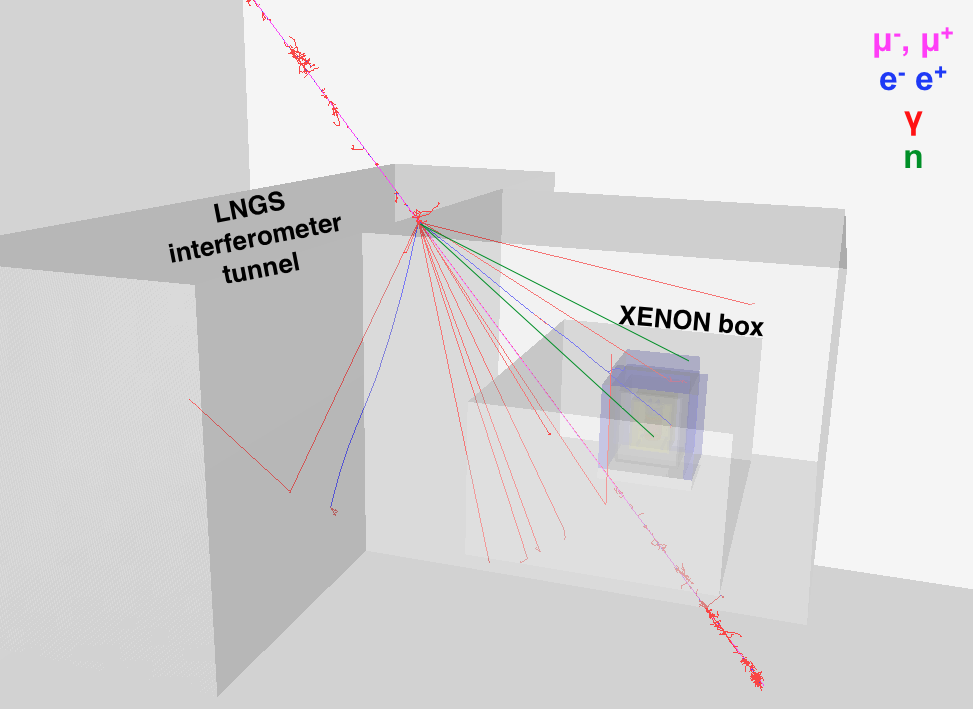
\includegraphics[width=1.0\linewidth]{plots/NRmuons/MuonSimulation_withNeutrons.png}
\caption[An example of a muon interaction in the GEANT4 simulation]{The GEANT4 model of the experimental site of XENON100 for simulations of the muon-induced neutron background. An example of a muon interaction is shown, producing two neutrons and an electromagnetic shower in the rock. One neutron is stopped by the water shield, and another one penetrates into the detector volume.}
\label{figMuonSimulation}
\end{figure}

\begin{figure}[!t]
\centering
%\subfigure[]{
%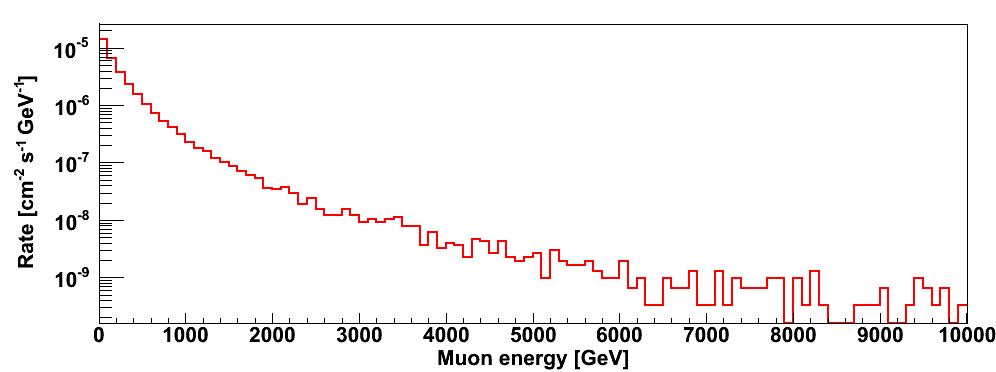
\includegraphics[width=0.9\linewidth]{plots/NRmuons/MuonSpectrum_wide.png}
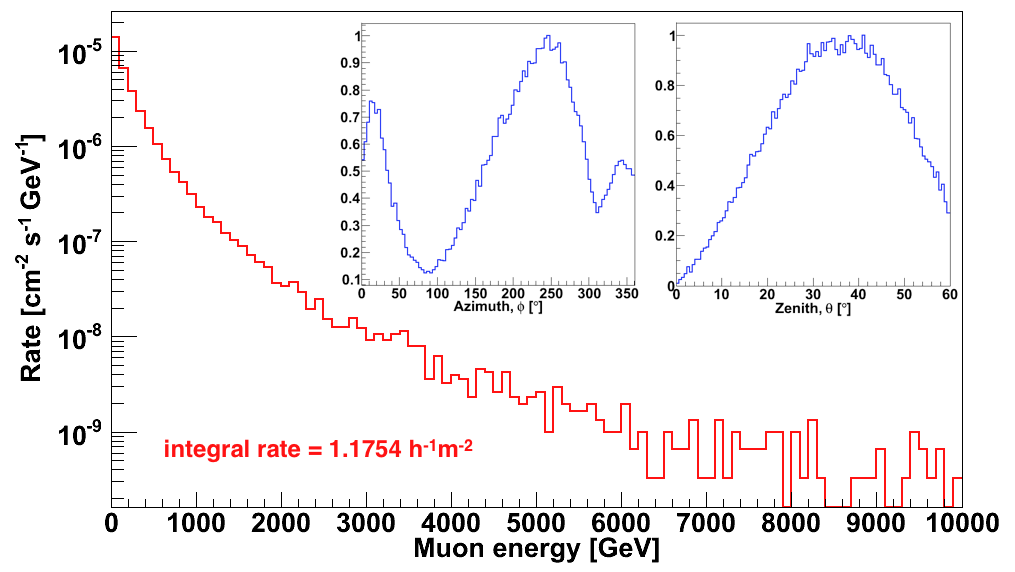
\includegraphics[width=0.8\linewidth]{plots/NRmuons/MuonSpectraAll.png}
%\label{figMuonSpectra_1}}
%\subfigure[]{
%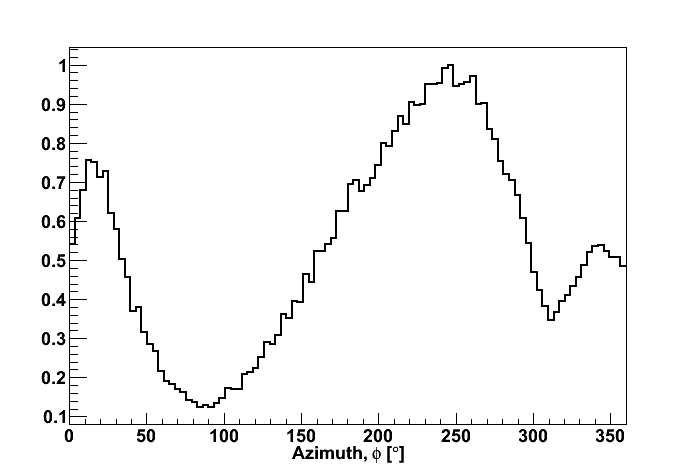
\includegraphics[width=0.475\linewidth]{plots/NRmuons/MuonAzimuth1.png}
%\label{figMuonSpectra_2}}
%\subfigure[]{
%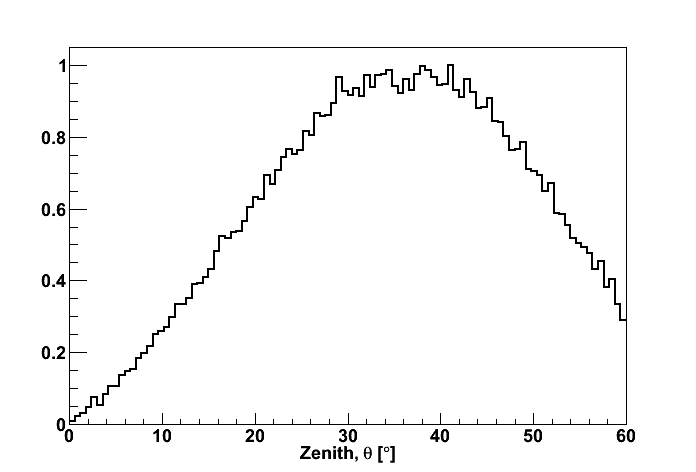
\includegraphics[width=0.475\linewidth]{plots/NRmuons/MuonZenith1.png}
%\label{figMuonSpectra_3}}
\caption[Energy and angular spectra of the muons at LNGS from simulations with MUSIC and MUSUN]{Energy and angular (inserts) spectra of the muons at LNGS from simulations with MUSIC and MUSUN. The small contribution of muons with zenith angle $>$60$^{\circ}$ has been ignored for the simulations with GEANT4.}
\label{figMuonSpectra}
\end{figure}

In order to simulate the muon-induced background, the GEANT4 model described in Section~\ref{secGeant4model} has been updated with the rock and the concrete shell of the experimental hall, taking into account a thickness of 5~m. Gran Sasso rock consists mainly if CaCO$_{3}$ and MgCO$_{3}$ and has an average density of (2.71$\pm$0.05)~g/cm$^{3}$~\cite{LNGSrock}. The interferometer tunnel, where the detector is located, has been simplified to a `cubic' model, and the structure of the experimental `box' has been ignored. The model is shown in Fig.~\ref{figMuonSimulation}, together with an example of a muon interaction in the rock of the laboratory, which generates two neutrons and an electromagnetic shower.

A muon flux of 1.1754 h$^{-1}\cdot$m$^{-2}$ has been assumed for the simulations, as measured by MACRO~\cite{MuonIntensity_MACRO} and LVD~\cite{MuonIntensity_LVD}. The seasonal variation of the muon intensity~\cite{MuonSeasonalModulation} has been ignored. The muon energy and angular spectra have been simulated with the MUSIC~\cite{MUSIC} and MUSUN~\cite{MUSICandMUSUN} packages, and are shown in Fig.~\ref{figMuonSpectra}. The average muon energy is 273~GeV, which is in a good agreement with the simulations from Ref.~\cite{MeiHime} and measurements reported in Ref.~\cite{MuonIntensity_MACRO}.
The $\mu^{+}$/$\mu^{-}$ ratio equals 1.4, as shown by recent observations for high energy muons~\cite{MuonRatio}. Most of the muons are coming with zenith angle $<$60\%.

\begin{table}[!b]
\centering
\caption[Muon-induced neutron production in the detector and shield components]{Muon-induced neutron production in the detector and shield components. The left column shows the origin material of all neutrons that produce nuclear recoils in the target volume, and the right one only of those neutrons that contribute to the nuclear recoil background, after the analysis cuts (energy, no coincidence with electronic recoils, veto coincidence cut, etc.) have been applied. The 'other' materials include the copper parts of the TPC structure, PMTs and cables, the resistor chain connecting the field shaping rings, cryostat support bars made from 316Ti stainless steel, support rings for the electrode meshes, and the diving bell. Neutron production in liquid xenon is relatively high, but they do not contribute to the nuclear recoil background }
\label{tabNeutronProductionMuons}
%\vspace{0.2cm}
\begin{tabular}{>\footnotesize{l} | >\footnotesize{c} | >\footnotesize{c}}
\hline
Component		      & \multicolumn{2}{>\footnotesize{c}}{Neutron production [\%]} \\
  		     		      & all neutrons & background  \\
\hline
Rock and concrete 				&  0.18		&  5		\\
Water shield					&  0.02		&  5		\\
Lead shield 					&  5.88 		&  15		\\
Polyethylene shield 				&  1.51		&  5		\\
Copper shield 					&  32.64		&  55		\\
Cryostat				 		&  3.18		& negligible	\\
Detector PTFE 					&  5.13		&  10 	\\
Liquid xenon 					&  46.30		&  5		\\
Other						&  5.16		& negligible	\\
\hline
\end{tabular}
\end{table}

The propagation of the high energy muons has been performed  with GEANT4.9.3.p01 using the `QGSP\_BIC\_HP' physics list \cite{G4_PhysicsList}, which is based on a quark gluon string model for high energy hadronic interactions~\cite{QGSP}, with a data driven high precision neutron package to transport neutrons below 20~MeV down to thermal energies. For primary protons and neutrons with energies below 10~GeV, is uses the GEANT4 binary cascade, which better describes production of secondary particles in interactions with nuclei. Inelastic interactions with matter of ions up to a few GeV/nucleon are modeled using a binary light ion cascade. The direct interaction between muons and nuclei is modeled with the `G4MuNuclearInteraction' process~\cite{G4MuNuclInteraction}, which handles it by producing virtual photons and treating them as a combination of $\pi^{+}$ and $\pi^{-}$ interactions using parametrized models.

About 0.3~billion muons have been simulated, which corresponds to live time of 185.5~years, and results in a statistical uncertainty of $\sim$10\%. The validation of the muon-induced neutron production has been performed via comparison with experimental data from NA55~\cite{MuonNeutronProd_NA55}, resulting in a factor of $\sim$2 overproduction by a Monte Carlo simulation, and via comparison with the data measured by the ZEPLIN-II experiment~\cite{MuonNeutronProd_ZeplinAraujo, MuonNeutronProd_Zeplin}, which indicated a controversial factor of $\sim$2 underproduction by GEANT4. These results have been used to set the systematic uncertainty of the simulations for GEANT4 by assigning asymmetric error bars.

\begin{figure}[!b]
\centering
\subfigure[single scatter events]{
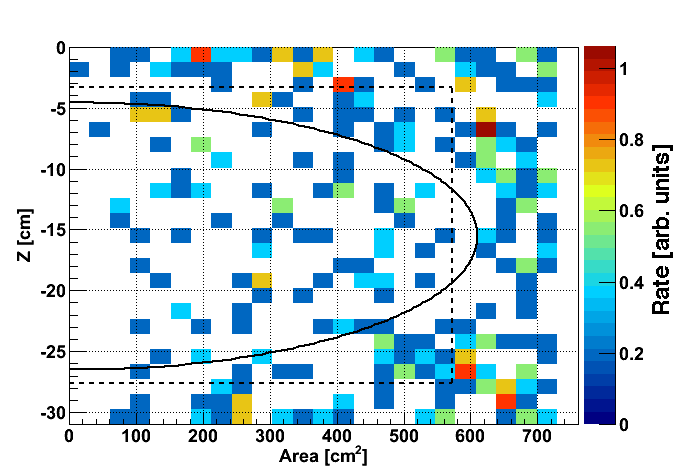
\includegraphics[width=0.475\linewidth]{plots/NRmuons/MuonInduced_AZ_SingleScatters_PassiveVeto_ArbUnits.png}
\label{figMuonInducedAZ_1}}
\subfigure[multiple scatter events]{
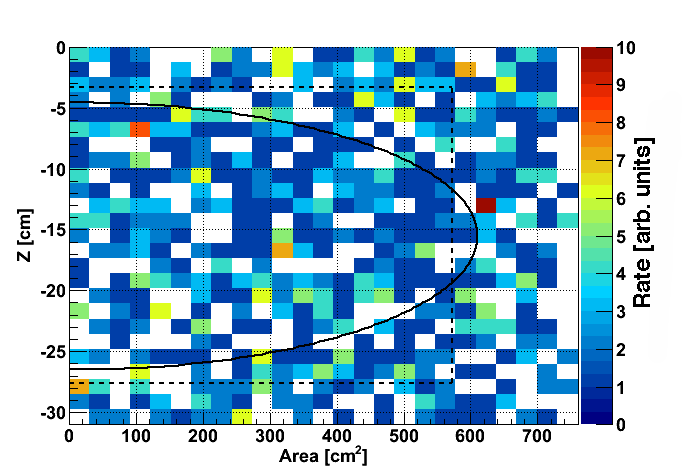
\includegraphics[width=0.475\linewidth]{plots/NRmuons/MuonInduced_AZ_MultipleScatters_PassiveVeto_ArbUnits.png}
\label{figMuonInducedAZ_2}}
\caption[Spatial distribution of nuclear recoils from muon-induced neutron interactions]{Spatial distribution of single scatter (a) and multiple scatter (b) muon-induced neutron interactions. The position of multiple scatter events shown here is defined by the position of the interaction with the highest energy deposition. The dashed line shows the 40~kg fiducial volume used for the first dark matter search (see Section~\ref{secRun07}), and the solid line indicates a 30~kg fiducial volume optimized for electronic recoil background reduction (see Section~\ref{secDetectorMaterials}). The rather uniform distribution shows that fiducialization is inefficient for the reduction of muon-induced neutron background.}
\label{figMuonInducedAZ}
\end{figure}

\begin{figure}[!b]
\centering
\subfigure[]{
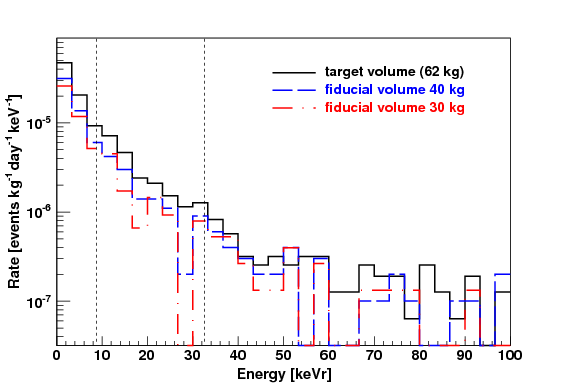
\includegraphics[width=0.475\linewidth]{plots/NRmuons/MuonInducedBG_PassiveVeto_withFV40andFV30.png}
\label{figMuonInducedBGspectra_1}}
\subfigure[]{
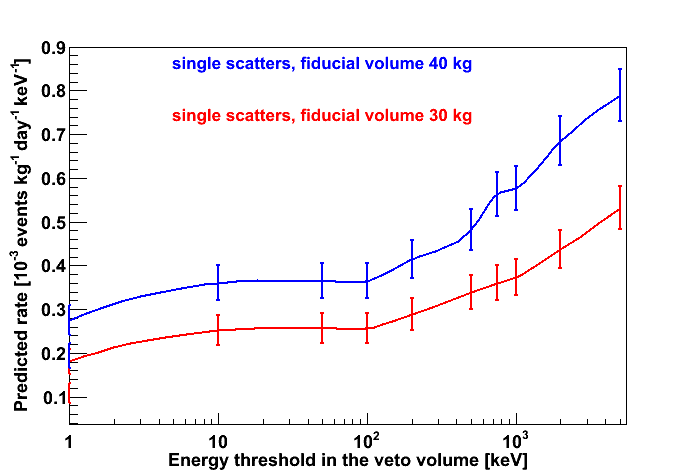
\includegraphics[width=0.475\linewidth]{plots/NRmuons/VetoReduction_Muons-NRVC_FV40andFV30.png}
\label{figMuonInducedBGspectra_2}}
\caption[Predicted spectra of nuclear recoils due to muon-induced neutrons, and the efficiency of the veto coincidence cut for background reduction as a function of energy]{Predicted spectra of nuclear recoils due to muon-induced neutrons (a), and the efficiency of the veto coincidence cut for background reduction as a function of energy (b). The error bars reflect the $\sim$10\% statistical uncertainty of the Monte Carlo simulation with GEANT4. Veto coincidence cut with the measured volume averaged threshold of 100~keV$_{ee}$ reduces the background rate in a fiducial volume by a factor of $\sim$2. }
\label{figMuonInducedBGspectra}
\end{figure}

The muon-induced neutron production in different materials is presented in Table~\ref{tabNeutronProductionMuons}. It has been calculated for all neutrons that produce nuclear recoils  in the target volume (left column), and only for those neutrons that have a `pure' single scatter nuclear recoil signature in the low energy region of interest and contribute to the background (right column). 
%Neutrons produced outside of the detector shield contribute less than the ones produced inside the significantly to the total muon-induced background, as they are efficiently stopped by the water or polyethylene shield layers.
The production of neutrons in liquid xenon is relatively high. However, they do not contribute significantly to the nuclear recoil background dangerous for the experiment, as they are coincident with high energy deposits from the primary muon or an associated electromagnetic cascade. The largest contribution (55\%) to the background is from neutrons generated in the innermost shield layer made from copper.

The spatial distribution of nuclear recoils is shown for single and multiple scatter events in Fig.~\ref{figMuonInducedAZ}. The position of the multiple scatter interactions has been defined by the position of the interaction with the highest energy deposition. The event distribution is rather uniform, hence fiducialization of the target is not very efficient to reduce the background from this source. This is illustrated by the energy spectra of nuclear recoils the entire liquid xenon target and in 40~kg and 30~kg fiducial volumes, shown in Fig.~\ref{figMuonInducedBGspectra_1}. 

Since the muon-induced neutron production is often followed by an electromagnetic cascade, and by high energy deposition from the incident muon, the background can be reduced by applying a veto coincidence cut. Electronic and nuclear recoils in the veto volume cannot be distinguished as it is done in the TPC based on the S2/S1 ratio, hence all energy depositions in the veto volume have been summed up, taking into account the relative scintillation efficiency for nuclear recoils, as described in Section~\ref{secLeff}. The efficiency of this cut as a function of the energy deposited in the veto volume is illustrated in Fig.~\ref{figMuonInducedBGspectra_2}. A veto coincidence cut with the measured volume averaged threshold of 100~keV$_{\mathrm{ee}}$ (see Section~\ref{secVetoEfficiencyMeasurement}) reduces the background rate in a fiducial volume by a factor of $\sim$2. 

The muon-induced background rates, predicted for the energy range 8.7$-$32.6~keV$_{\mathrm{nr}}$ used in the analysis of the data from the commissioning run in Fall 2009 (run07~\cite{xe100-run07}, see Section~\ref{secRun07}), are presented in Tables~\ref{tabMuonBGrates_1} and \ref{tabMuonBGrates_2}, without and with veto coincidence cut, respectively. Due to the quasi-exponential shape of the nuclear recoil spectra, falling off at higher energies (see Fig.~\ref{figMuonInducedBGspectra_1}), the increase of the background rate due to an increased upper analysis threshold, e.g. 44.8~keV$_{\mathrm{nr}}$ as used in the analysis of the first science run (run08~\cite{xe100-run08}, see Section~\ref{secRun08}), is not significant.

\begin{table}[!h]
\centering
\caption[Predicted background rate of nuclear recoils in the energy region of interest due to muon-induced neutrons, without veto cut]{Predicted background rate of nuclear recoils in the energy range 8.7$-$32.6~keV$_{\mathrm{nr}}$ due to muon-induced neutrons, {\it without veto cut}. The statistical error of the GEANT4 simulation is $\sim$1\%. A factor of 2 systematic uncertainty of the neutron production with GEANT4 is assumed from the validation via comparison of simulations and measured data for NA55~\cite{MuonNeutronProd_NA55} and ZEPLIN-II~\cite{MuonNeutronProd_ZeplinAraujo, MuonNeutronProd_Zeplin} experiments.}
\label{tabMuonBGrates_1}
\begin{tabular}{>\footnotesize{l} | >\footnotesize{c} | >\footnotesize{c} | >\footnotesize{c} | >\footnotesize{c}}
\hline
				      		& \multicolumn{4}{>\footnotesize{c}}{Predicted background rate [year$^{-1}$]} \\
Volume 		     			& 62~kg 					& 48~kg  					& 40~kg 					& 30~kg \\
\hline
all events 					& 6.73$^{+6.73}_{-3.37}$  	& 5.04$^{+5.04}_{-2.02}$ 		& 3.79$^{+3.79}_{-2.40}$ 		& 2.80$^{+2.80}_{-1.40}$ \\
single scatter events			& 1.95$^{+1.95}_{-0.98}$		& 1.20$^{+1.20}_{-0.60}$ 		& 0.84$^{+0.84}_{-0.42}$		& 0.55$^{+0.55}_{-0.28}$ \\
multiple scatter events		& 4.79$^{+4.79}_{-2.40}$ 		& 3.83$^{+3.83}_{-1.92}$ 		& 2.95$^{+2.95}_{-1.48}$		& 2.25$^{+2.25}_{-1.13}$ \\
double scatter events		& 1.61$^{+1.61}_{-0.81}$ 		& 1.15$^{+1.15}_{-0.60}$ 		& 0.83$^{+0.83}_{-0.42}$		& 0.58$^{+0.58}_{-0.29}$ \\
\hline
\end{tabular}
\end{table}

\begin{table}[!h]
\centering
\caption[Predicted background rate of nuclear recoils in the WIMP-search energy range due to muon-induced neutrons, with veto coincidence cut]{Predicted background rate of nuclear recoils in the energy range 8.7$-$32.6~keV$_{\mathrm{nr}}$ due to muon-induced neutrons, {\it with veto coincidence cut} (volume averaged energy threshold 100~keV$_{\mathrm{ee}}$).}
\label{tabMuonBGrates_2}
\begin{tabular}{>\footnotesize{l} | >\footnotesize{c} | >\footnotesize{c} | >\footnotesize{c} | >\footnotesize{c}}
\hline
				      		& \multicolumn{4}{>\footnotesize{c}}{Predicted background rate [year$^{-1}$]} \\
Volume 		     			& 62~kg 					& 48~kg  					& 40~kg 					& 30~kg \\
\hline
all events 					& 2.48$^{+2.48}_{-1.24}$ 		& 1.84$^{+1.84}_{-0.92}$ 		& 1.40$^{+1.40}_{-0.70}$ 		& 1.05$^{+1.05}_{-0.53}$ \\
single scatter events			& 0.80$^{+0.80}_{-0.40}$		& 0.51$^{+0.51}_{-0.26}$ 		& 0.35$^{+0.35}_{-0.18}$		& 0.23$^{+0.23}_{-0.12}$ \\
multiple scatter events		& 1.68$^{+1.68}_{-0.84}$ 		& 1.33$^{+1.33}_{-0.67}$ 		& 1.06$^{+1.06}_{-0.53}$		& 0.82$^{+0.82}_{-0.41}$ \\
double scatter events		& 0.61$^{+0.61}_{-0.31}$ 		& 0.44$^{+0.44}_{-0.22}$ 		& 0.32$^{+0.32}_{-0.16}$		& 0.21$^{+0.21}_{-0.11}$ \\
\hline
\end{tabular}
\end{table}



%\begin{figure}[!h]
%\begin{center}
%\begin{tabular}{cc}
%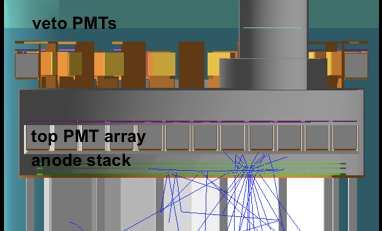
\includegraphics[width=0.5\linewidth]{plots/LCEs2/G4_S2simulation.png}
%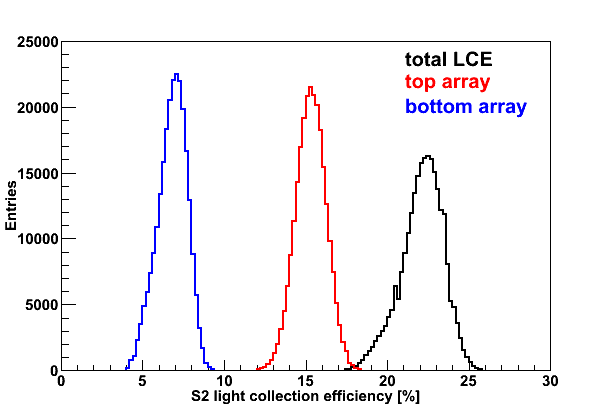
\includegraphics[width=0.5\linewidth]{plots/LCEs2/LCE_S2_comparison.png}
%\end{tabular}
%\caption{Monte Carlo simulation of the proportional scintillation signal with GEANT4.}
%\label{figLCEs2}
%\end{center}
%\end{figure}
